\documentclass[a4paper]{article}
%\include{amsfonts}
\usepackage{amssymb,amsmath,amsthm,latexsym,epsfig,euscript,multicol}
% \usepackage{enumitem}
\usepackage{graphicx}
\usepackage{float}
\usepackage[margin=2cm]{geometry}
\usepackage{hyperref}

%\usepackage[utf8x]{inputenc}
\usepackage[spanish]{babel}% idioma castellano
\graphicspath{{fig/}}

% Caracteres especiales
\def\A{\mathbb{A}}
\def\C{\mathbb{C}}
\def \N{\mathbb{N}}
\def \P{\mathbb{P}}
\def \Q{\mathbb{Q}}
\def \R{\mathbb{R}}
\def \Z{\mathbb{Z}}

\def\zC{\mathbb{C}}
\def \zN{\mathbb{N}}

\def \zQ{\mathbb{Q}}
\def \zR{\mathbb{R}}
\def \zZ{\mathbb{Z}}

%  Ejercicio:
\newtheorem{ejer}{Unidad}
\newcommand{\bej}{\begin{ejer} \rm}
\newcommand{\fej}{\end{ejer}}


%
\def\d{\displaystyle}

%Encabezado y pie de página
\usepackage{fancyhdr} % Headers and footers
\setlength{\headwidth}{16.5cm}
\pagestyle{fancy} % All pages have headers and footers


\renewcommand{\headrulewidth}{1.5pt}


\renewcommand{\footrulewidth}{1.5pt}

% \fancyhead{} % Blank out the default header
% \fancyfoot{} % Blank out the default footer
\fancyhead[L]{Ejercicios complementarios del taller de Python}
% \fancyhead[R]{{\small Departamento de Física, FCEN, UBA}}% Custom header text
\fancyfoot[R]{\thepage} % Custom footer text
\fancyfoot[L]{FIFA}


%\topmargin-2cm \vsize 29.5cm \hsize 21cm
%\setlength{\textwidth}{16.5cm} \setlength{\textheight}{23.5cm}
%\setlength{\oddsidemargin}{0.0cm}
%\setlength{\evensidemargin}{0.0cm}

%\linespread{1.4cm}
\usepackage{setspace}
 \onehalfspacing

%-------------------------------------------------------------------------------------------------
%-------------------------------COMIENZA EL TEXTO-------------------------------------------------
%-------------------------------------------------------------------------------------------------
\begin{document}
\thispagestyle{empty}

% \vskip 1cm

% \centerline{{\small \textit{Departamento de Física}}}
% \centerline{{\small \textit{Facultad de Ciencias Exactas y Naturales }}}
% \centerline{{\small \textit{Universidad de Buenos Aires}}}
% \vskip 1cm

\centerline{{\bf\Large{Ejercicios complementarios del taller de Python}}}

\centerline{{\ttfamily Talleres FIFA (Federación Interestudiantil de Físicos de Argentina)}}

\begin{figure}[H]
 \centering
   
\includegraphics[width=0.3\textwidth]{logos_python_fifa.png}
 \label{FIFA}
 \end{figure}

\bigskip


\textbf{Observación}:
En caso de que el IDE de sus computadoras no funcione, se puede probar programar online en la web: \url{https://www.python.org/shell/}
%https://cloud.sagemath.com/#settings
%https://www.pythonanywhere.com

\textbf{Observación 2}:
Estos ejercicios en general son menos guiados que los anteriores, y por ende más complejos. No teman buscar en internet.

\bigskip
\centerline{\bf Ejercicios propuestos}
\bigskip

\begin{enumerate}
	\item \texttt{es\_primo($n$)}: devuelve True si el input es un número primo. False en caso contrario.
	\item \texttt{factorial($n$)}: devuelve el factorial del input $n$. Recordar que el factorial se define: $n! = n\cdot(n-1)\cdot(n-2)\cdot \,\ldots\, \cdot1$
	\item \texttt{absoluto($x$)}: devuelve el valor absoluto del input $x$. Si $x<0$ debería devolver $-x$ y si $x\ge 0$ debería devolver $x$.
	\item \texttt{norma(x, y, z)}: devuelve la distancia euclídea entre el punto elegido y el origen de coordenadas
		\begin{itemize}
			\item modifique la función para que reciba un único parámetro v, que sea una tupla o lista de largo 3.
			\item extienda esta función para que reciba dos puntos y calcule la norma del vector que los une.
			\item puede extender la función para que calcule otras normas no euclídeas.
		\end{itemize}
	\item \texttt{perp(v1, v2)}: devuelve True si los vectores son perpendiculares y False si no lo son (recordar que es fácil ver si dos vectores son perpendiculares viendo su producto interno: $\vec{v}\cdot \vec{w} = v_1w_1 + v_2w_2 + v_3 w_3$. )
		\begin{itemize}
			\item Generalice a dos vectores de largo $N$, con un $N$ arbitrario.
		\end{itemize}
	\item \texttt{prod\_vectorial(v, w)} devuelve el producto vectorial $\vec{v}\times \vec{w} = (v_2 w_3 - v_3 w_2; v_3 w_1 - v_1 w_3; v_1 w_2 - v_2 w_1)$. Para verificar la función pueden verificar que $(1;0;0)\times (0;1;0) = (0;0;1)$ (esto es la regla de la mano derecha: $\hat{i} \times \hat{j} = \hat{k}$, para los que la conozcan).
	\item Considere la serie de Taylor de la función exponencial $f(x)=e^x=\sum\limits_{n=0}^{\infty} (x^n) / n!$. Como esta suma es infinita se imaginarán que tarda infinito tiempo en converger al valor con error nulo. No obstante, cada término que se calcula acerca la estimación al valor real. El objetivo de este ejercicio es ver la convergencia de esta serie, para realizarlo les conviene tener algunas de las funciones de los ejercicios anteriores a mano.\\
		Escriba una función \texttt{exp\_taylor($x$, $N$)} que reciba como parámetros el valor de $x$ donde evaluar la exponencial y $N$ siendo el orden de precisión deseado (es decir que la sumatoria en vez de ser hasta $\infty$ será hasta $N$) y devuelva el resultado de la sumatoria parcial obtenida.\\
		Luego compare con el valor "real" de la función (que pueden obtener, por ahora, usando una calculadora o Google o Mathematica. La próxima clase veremos de donde podemos obtener el valor desde python). Por ejemplo: Se quiere ver la convergencia para $x=4$, entonces buscamos el valor posta $e^4 \approx 54.5981500331$, y para ver el error hacemos: $\textup{error} = |\,54.5981500331 - \texttt{exp\_taylor(4, N)}\,|$.
		La pregunta que se quiere saber es, a qué orden necesito hacer la cuenta para encontrar una aproximación que difiera del valor real en menos de $0.1$. Y $0.01$? $0.001$? etc\ldots.\\
		Esto va a estar bueno cuando aprendamos a hacer gráficos, vamos a poder ver el error en función del orden de aproximación.

	\item \texttt{verificar\_nombre(str)}: Esta función va a recibir un string, y va a verificar si es compatible como nombre de archivo devolviendo True o False. Vamos a aceptar nombres solamente si \emph{no} contienen los caracteres: [ ] ( ) \{ \} , / ; . *

	\item ¡Adivina un número del uno al diez! Defina un número del 1 al 10, luego pídale al usuario que ingrese un número. Si adivina el número que muestre un mensaje de felicitaciones y si no que siga intentando.\\
		Para esto puede usar la función \texttt{input}. Deberá buscar en internet o la documentación de esta función, en particular para ver qué tipo de dato devuelve esta función (si es un \texttt{int, str, \ldots}).
\end{enumerate}

\begin{figure}[H]
 \centering
 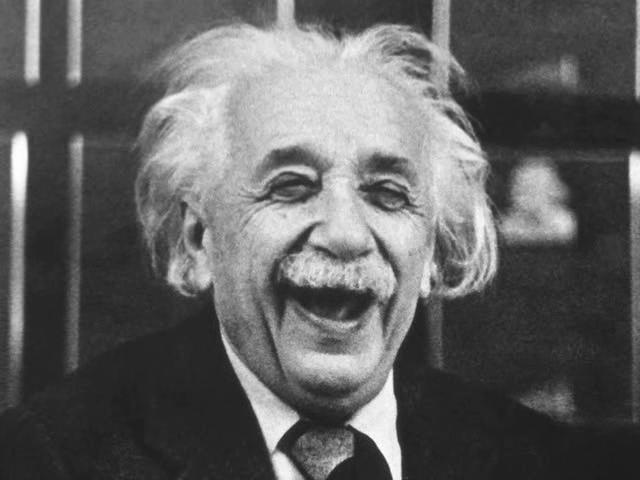
\includegraphics[width=0.4\textwidth]{einstein.jpeg}
 \label{Einstein}
 \end{figure}


\end{document}
